\section{RC Week 4}
\subsection{Building a C++ program}
\begin{frame}{The problem of \textit{building} complex programs}
\vspace{-0.10in}
\begin{block}{\textit{Building} is different from \textit{compiling}}
	\vspace{-0.07in}
	\begin{itemize}
		\item Compiling refers to the process of translating code to binaries.
		\item Building is \textbf{piecing together} from its components.
		\item A program might depend on other package.
		\item A program might use a pre-compiled library.
		\item A program might involve more than one source files.
		\item A program might need to be built for different platform.
		\item Sometimes you not only needs to build just one executable, but also documentations / test suites / libraries for the sake of other programs.
	\end{itemize}
\end{block}
\vspace{-0.15in}
\begin{block}{How complicated is Linux kernel version 3.2?}
	\vspace{-0.07in}
	\begin{itemize}
		\item 37,626 – The number of files 
		\item 15,004,006 – The number of lines of code 
	\end{itemize}
\end{block}
\end{frame}

\begin{frame}{\textit{Building} a multi-file C++ program}
\begin{block}{The golden rule}
	\vspace{0.05in}
	\textrm{\textbf{\large{Each source file (\texttt{.cpp}, \texttt{.c}) compiles independently.}}}
\end{block}
\begin{block}{The \textit{building} process}
	\vspace{0.1in}
	\centering

	% Define block styles
	\tikzstyle{decision} = [diamond, draw, fill=blue!20, 
	text width=4.5em, text badly centered, node distance=3cm, inner sep=0pt]
	\tikzstyle{block} = [rectangle, draw, fill=blue!20, 
	text width=5em, text centered, rounded corners, minimum height=4em]
	\tikzstyle{line} = [draw, -latex']
	\tikzstyle{cloud} = [draw, ellipse,fill=red!20, node distance=3cm,
	minimum height=2em]
	
	\begin{tikzpicture}[node distance = 3cm, auto, scale=0.8, every node/.style={scale=0.8}]
	% Place nodes
	\node [block] (source) {Source \texttt{.cpp}};
	\node [draw,trapezium,trapezium left angle=70,trapezium right angle=-70, above of=source, node distance=2cm] (preproc) {Preprocessor};
	\node [block, above of=preproc, node distance=2cm] (prep) {Preprocessed Source \texttt{.cpp}};
	\node [draw,trapezium,trapezium left angle=70,trapezium right angle=-70, right of=prep, node distance=3cm] (compiler) {Compiler};
	\node [block, right of=compiler] (object) {Objects files \texttt{.o}};
	\node [block, below of=object] (outside) {Other Objects \texttt{.o}};
	\node [draw,trapezium,trapezium left angle=70,trapezium right angle=-70, right of=object] (linker) {Linker};
	\node [block, right of=linker] (executable) {exactuable};
	%\node [block, below of=decide, node distance=3cm] (stop) {stop};
	% Draw edges
	%\path [line] (source) -- (compiler);
	\path [line] (source) -- (preproc);
	\path [line] (preproc) -- (prep);
	\path [line] (prep) -- (compiler);
	\path [line] (compiler) -- (object);
	\path [line] (object) -- (linker);
	\path [line] (outside) -- (linker);
	\path [line] (linker) -- (executable);
	\end{tikzpicture}
\end{block}
\end{frame}

\begin{frame}{The \texttt{g++} tool chain}
\begin{block}{\texttt{g++} as a all-in-one tool}
	\vspace{-0.07in}
	\begin{itemize}
		\item Preprocessor, compiler and linker used to be separate.
		\item Now \texttt{g++} combines them into one.
		\item By default \texttt{g++} takes source files and generate executable.
		\item Using different switches you can perform individual step.
	\end{itemize}
\end{block}
\vspace{-0.15in}
\begin{block}{Options for \texttt{g++}}
	\vspace{-0.07in}
	\begin{description}[-O\{0123\}]
		\small
		\item[-o out] Name the output file as \texttt{out}. Outputs \texttt{a.out} if not present.
		\item[-std=] Specify C++ standard. Recommend \texttt{-std=c++11}.
		\item[-Wall] Report all warnings.
		\item[-O\{0123\}] Optimization level. \texttt{-O2} is the recommended for release.
		\item[-c] Only compiles the file (Can not take multiple arguments).
		\item[-E] Only pre-processes the file (Can not take multiple arguments).
	\end{description}
\end{block}
\end{frame}

\begin{frame}[fragile]{An example}
This example contains a ``main" source file accompanied with multiple other source files. All files are compiled separately into object files. We link some of them together and see what happens.

\vspace{0.04in}
\textit{Keep in mind variables/function must be first declared before used.}

\vspace{0.04in}
\texttt{$-->$ code/rc4build/main.cpp}
\inputminted{c++}{code/rc4build/main.cpp}
\end{frame}

\begin{frame}[fragile]{An example}
\label{example:dec_def}
\vspace{0.04in}
\texttt{$-->$ code/rc4build/odd.cpp}
\inputminted{c++}{code/rc4build/odd.cpp}

\vspace{0.04in}
\texttt{$-->$ code/rc4build/even.cpp}
\inputminted{c++}{code/rc4build/even.cpp}

\vspace{0.04in}
\texttt{$-->$ code/rc4build/sum.cpp}
\inputminted{c++}{code/rc4build/sum.cpp}
\end{frame}

\begin{frame}[fragile]{An example}
\texttt{$-->$ code/rc4build/prod.cpp}
\inputminted{c++}{code/rc4build/prod.cpp}

\vspace{0.04in}
\begin{small}
	The following file is a C source file. This file is given just for you to know you can do pretty weired things if you know the deal.
\end{small}

\texttt{$-->$ code/rc4build/sum\_large.c}
\inputminted{c++}{code/rc4build/sum_large.c}

\end{frame}

\begin{frame}[fragile]{An example}
We compile the source files one by one. 
\begin{minted}{text}
$ g++ -o main.o -c main.cpp
$ g++ -o odd.o -c odd.cpp
$ g++ -o even.o -c even.cpp
$ g++ -o sum.o -c sum.cpp
$ g++ -o prod.o -c prod.cpp
\end{minted}
Next one is compiled through gcc
\begin{minted}{text}
$ gcc -o sum_large.o -c sum_large.c
\end{minted}

Next step we are going to link (some of) them and execute it. Linking in \texttt{g++} is easy. If you supply \texttt{.o} files, \texttt{g++} will know that is should link them instead of compiling them.

Pay extra attention to compiler errors (actually linker errors), they are the most interesting part.

\end{frame}

\begin{frame}[fragile]{An example}
Now first standard examples
\begin{minted}{text}
$ g++ -o main main.o even.o sum.o && ./main
$ g++ -o main main.o even.o prod.o && ./main
$ g++ -o main main.o odd.o prod.o && ./main
\end{minted}

Now what if we link both \texttt{even.o} and \texttt{odd.o}
\begin{minted}{text}
$ g++ -o main main.o odd.o even.o prod.o && ./main
\end{minted}

Now what if we link both \texttt{prod.o} and \texttt{sum.o}
\begin{minted}{text}
$ g++ -o main main.o odd.o sum.o prod.o && ./main
\end{minted}

Now what if we leave out both \texttt{even.o} and \texttt{odd.o}
\begin{minted}{text}
$ g++ -o main main.o prod.o && ./main
\end{minted}

Now what if we leave out the \texttt{main.o} 
\begin{minted}{text}
$ g++ -o main even.o prod.o && ./main
\end{minted}

\end{frame}

\begin{frame}[fragile]{An example}
\framesubtitle{Surprises}

Now we introduce something crazy. The name of the function in \texttt{sum\_large.c} is really strange. But we just ignores that link its object file any way.
\begin{minted}{text}
$ g++ -o main main.o even.o sum_large.o && ./main
\end{minted}

Well it worked. The question is how on earth can this work. In fact \texttt{g++} is doing some crazy renaming when compiling your source code. The reason why they did this is understandable when you think about it in the later period of the course. 

Understanding linking actually allows you to do some crazy things. Try compiling the following file (with only one line of code) on your machine. 
\begin{minted}{text}
int main[-1u] = {1};
\end{minted}

It tooks quite long to finish. How large is the executable?

\end{frame}

\begin{frame}{Headers and inclusion}
\begin{block}{\texttt{\#include<>} : Why we need them?}
	\begin{itemize}
		\item Things must be declared before used.
		\item Each source file compiles independently. Needs a method to ``export" functions defined in one file to other files.
		\item Avoid repeating declarations. 
	\end{itemize}
\end{block}
\begin{block}{Preprocessing}
	\begin{itemize}
		\item Preprocessing is purely \textbf{textual}. 
		\item \texttt{\#include} simply copy the content.
		\item \textit{Conditional compilation directives }simply deletes unused branch. (\texttt{\#ifdef}, \texttt{\#ifndef}, \texttt{\#else}, ...)
	\end{itemize}
\end{block}

\end{frame}

\begin{frame}[fragile]{Header guards}
\framesubtitle{problem}
Whenever there is dependence of source files, there will be dependence of headers.

Consider the following \texttt{a.cpp}, \texttt{a.h}, \texttt{b.h} and \texttt{c.h}. Keep in mind that \textit{everything in C++ is allowed to have at most 1 definition during compilation.}

\begin{columns}
	\column{.5\textwidth}
	$-->$ \texttt{a.cpp}
\begin{minted}{c++}
#include "a.h"
#include "b.h"
int main() {...}
\end{minted}
	\column{.5\textwidth}
$-->$ \texttt{point.h}
\begin{minted}{c++}
struct Point{
    int x, y;
}
\end{minted}
\end{columns}
\vspace{0.2in}
\begin{columns}
	\column{.5\textwidth}
	$-->$ \texttt{a.h}
\begin{minted}{c++}
#include "point.h"
int area(Point a, Point b);
\end{minted}
\column{.5\textwidth}
$-->$ \texttt{b.h}
\begin{minted}{c++}
#include "point.h"
void circle(Point o, int r);
\end{minted}
\end{columns}
\end{frame}

\begin{frame}[fragile]{Header guards}
\framesubtitle{Solution}
The idea is to use a unique macro to guard a header.
\begin{itemize}
	\item Define that unique macro when the header is first included.
	\item Check if the macro is defined in future inclusion.
\end{itemize}

Now \texttt{point.h} becomes:

\begin{minted}{c++} 
#ifndef _POINT_H_
#define _POINT_H_
struct Point {int x, y;}
#endif
\end{minted}

The macro could be something else. Just don't use something common.

\end{frame}

\begin{frame}{Build systems}
\structure{The need for a build system}
\begin{itemize}
	\item Build process is complicated, avoid type every command.
	\item Project have dependence, need to manage dependence
	\item Compile minimum amount of code possible upon update.
	\item Many other reasons, abstract out actual compiler, compile for different platform / target.
\end{itemize}
\structure{Choices of build systems}
\begin{description}[GNU/make]
	\item[GNU/make] Our choice of make system. It has a very long history.
	\item[CMake] A modern make system used by CLion and many other projects. Very flexible and reliable. It is also a cross platform solution.
	%\item[MSBuild] Build system used by Visual Studio.
\end{description}
\end{frame}

\begin{frame}{\textit{Makefile} and it's syntax}
\structure{The \textit{Makefile}}
\begin{itemize}
	\item The executable for GNU/make is simply \texttt{make}
	\item \texttt{make} requires a file that describes the building process. Such file is named \texttt{Makefile}. 
	\item \texttt{Makefile} is made up of \textit{targets}. A target can depend on other target, or some file.
\end{itemize}
\structure{Syntax}

The following syntax defines a target. Note the \texttt{tab} key.

\vspace{0.1in}

\texttt{\textit{TargetName} : Dep1 Dep2 file1.o file2.o}

\texttt{\keys{\tab} \textit{Command1-to-run}}

\texttt{\keys{\tab} \textit{Command2-to-run}}

\end{frame}

\begin{frame}{\textit{Makefile} : Example}
This is a \texttt{Makefile} for our previous example.
\texttt{$-->$ code/rc4build/Makefile}
\inputminted{make}{code/rc4build/Makefile}
\end{frame}

% \begin{frame}[fragile]{Exercise}
% Write a \texttt{Makefile} for your project 2.

% \begin{minted}{bash}
% g++ -std=c++11 -Wall -o test test.cpp recursive.cpp p2.cpp
% \end{minted}

% Send your Makefile to \texttt{syqian@sjtu.edu.cn} or submit a pull request to \texttt{ve280/ve280}.

% \end{frame}

\begin{frame}[fragile]{CMake}
CMake stands for Cross-platform Make. You're required to use CMake if you're using CLion.

The build process has one step if you use a Makefile, namely typing “make” at the command line. For CMake, there are two steps\footnote{\url{https://prateekvjoshi.com/2014/02/01/cmake-vs-make/}}: 
\begin{enumerate}
    \item Setup your build environment.
    \item Perform the actual build in the selected build system.
\end{enumerate}

Commands:
\begin{minted}{bash}
mkdir build && cd build
cmake ..
make
\end{minted}

\end{frame}

\begin{frame}[fragile]{CMakeList.txt}

Example CMakeList.txt

\begin{minted}[breaklines]{cmake}
cmake_minimum_required(VERSION 3.8)
project(surfaces)
set(CMAKE_CXX_STANDARD 11)
find_package(OpenCV REQUIRED)
set(CMAKE_CXX_FLAGS_RELEASE "${CMAKE_CXX_FLAGS_RELEASE} -march=native -ffast-math")
add_executable(main main.cpp utils.cpp)
target_link_libraries(main ${OpenCV_LIBS})
\end{minted}

\end{frame}

\subsection{Review of C++}

\begin{frame}{Review of C++}

\begin{itemize}
	\item Standardized C++ and Undefined Behaviors.
	\item Declaration versus Definition.
	\item lval versus rval.
	\item References.
	\item Function argument passing.
	\item const modifier.
	\item Function pointers.
\end{itemize}

\end{frame}

\begin{frame}{Standardized C++}
Once upon the time, programming languages are just conventions, design choices made by the language creator. 

\structure{The standardize process}
\begin{itemize}
	\item Establishes program syntax, what are acceptable and what are syntax errors?.
	\item Language semantics, what's the ``meaning" of an expression / language construct.
	\item Behavior, what are the expected behavior and what are undefined and left to the choice of compilers ...
	\item Standard library, what to include and what's the implementation constraint.
\end{itemize}
The latest standard is C++17 (3/21/2017). Major standards are C++98, C++03, C++11, C++14. C++ after C++11 is generally considered ``modern C++". 
\end{frame}

\begin{frame}{Online reference for \texttt{std::to\_string()}}

The following information comes from \url{http://www.cplusplus.com/reference/string/to\_string/}

\begin{figure}
	\centering
	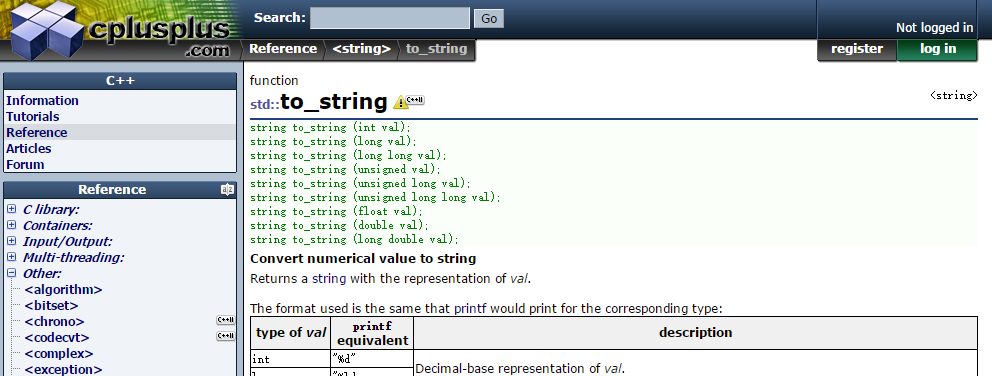
\includegraphics[scale=0.4]{fig/rc4_tostring}
	\caption{Online reference for \texttt{C++11} library function \texttt{to\_string}}
	\vspace{-0.2in}
\end{figure}

\begin{itemize}
	\item Notice the \texttt{C++11} sign.
	\item Notice the overloads supported by this function.
\end{itemize}
\end{frame}

\begin{frame}{\textit{Undefined Behaviors}}
One outcome from the standardize process is that, almost every true-or-false question about the C++ program can be answered with one of the following decisively. It is either YES, NO, or more importantly \textbf{undefined behavior} (\textit{UB} for short).

Undefined behaviors are program whose output depends on a specific platform, or a specific implementation of the compiler. You should always remember the following:
\begin{itemize}
	\item It's an absolute waste of time trying to figure out what will happen given an code that contains UB.
	\item It's dangerous and to write code that contains UB.
	\item Anyone who test you with UB, is both stupid and ignorant.
\end{itemize}

There is a reason why UB exists. It's not that the committee doesn't know how to eliminate them, but they leave room for pretty impressive \textit{compiler optimizations}.
\end{frame}

\begin{frame}{Undefined Behaviors}
Any (zero or more) of the following may happen if you trigger any of undefined behaviors:

\begin{itemize}
	\item The compiler may refuse to compile.
	\item The compiler still compiles, but throw you an warning
	\item The compiler compiles silently.
	\item Your program crashes when executed.
	\item Your program malfunctions when executed.
	\item The compiler deletes all your photos.
	\item 72 fairies come out of your screen and dance around you.
	\item \textbf{\textcolor{red}{Your program works perfectly.}}
\end{itemize} 

\textbf{It's your job to avoid UB}. We may refuse to answer the ``why my program works locally but crashes on OJ" type of question.
\end{frame}

\begin{frame}[fragile]{Undefined Behaviors}
\framesubtitle{Common cases}


- Integer overflow (No, it's not guaranteed to be negative!)
\begin{minted}{c++}
int x = INT_MAX; x++; 
\end{minted}

- Dereferencing \texttt{nullptr} (No, it's not guaranteed to be crash!)
\begin{minted}{c++}
int* x = nullptr; *x = 2;
\end{minted}

- Array out-of-bound (Even taking address is UB!)
\begin{minted}{c++}
int x[10] = {0};  x[10] = 1; int* x = &(x[11]);
\end{minted}



- Dangling references (You could still get correct value)
\begin{minted}{c++}
int* x = int[10]; x[3] = 5; delete[] x; cout << x[3]; 
int* f(int t) {return &t;} int* x = f(10); cout << *x;
\end{minted}

% - Evaluation order and side effect :)
% \begin{minted}{c++}
% int i = 0; i = i++; // Yes that's UB
% int j = i++ + ++i; // Yes that's UB too
% f(j = i, i = j); // That's right UB again.
% \end{minted}

\end{frame}

\begin{frame}[fragile]{\textit{Declaration} versus \textit{Definition}}

Consider writing a declaration for the following \texttt{add} function.
\begin{minted}{c++}
int add(int x, int y) {return x + y;}
\end{minted}
No doubt above is a function definition. We first write
\begin{minted}{c++}
int add(int x, int y);
\end{minted}
Well, that's a right answer. But we could also do
\begin{minted}{c++}
int add(int elephant, int haskell);
\end{minted}
Suprised? Well it makes sense since changing formal arguments doesn't change the function at all! $f(x) = x$ and $f(z) = z$ are the same function. But we could push this even further!
\begin{minted}{c++}
int add(int, int);
\end{minted}
This will work as well.
\end{frame}

\begin{frame}[fragile]{\textit{lval} and \textit{rval}}
Compare the following 2 expression, suppose \text{arr} is an array of integers
\begin{enumerate}
	\item \mintinline{c}{arr[10]}
	\item \mintinline{c}{arr[10] + arr[1]}
\end{enumerate}
They both have the type \texttt{int} of course. 
\begin{itemize}
	\item \mintinline{c}{int *p = &(arr[10]);} makes sense.
	\item \mintinline{c}{int *p = &(arr[10] + arr[1]);} gives you compile error.
\end{itemize}  
Further more
\begin{itemize}
	\item \mintinline{c}{arr[10] = 10;} makes sense.
	\item \mintinline{c}{arr[10] + arr[1] = 20;} doesn't
\end{itemize} 
Clearly the two expression are ``different" in some sense. How? Think about memory! The first kind is called \textit{left values} and the second is called \textit{right values}. (Those are not technical definitions.)
\end{frame}

\begin{frame}[fragile]{References}

\textit{What we discuss here applies only to non-const references!}

Lvals always corresponds to a fixed memory region. This gives rises to a special construct called \textit{references}. 

\begin{minted}{c++}
int a = 1, b[10] = {2};
int& ra = a; int& rb3 = b[3];
a = 10; /* ra reads 10 */ ra = 20; // a reads 20
\end{minted}

Think about references as aliases. Essentially, you are giving the memory region associated with \texttt{a} an extra name \texttt{ra} (memory region given by \texttt{b[3]} an extra name \texttt{rb3}). 

Try resist the temptation to think reference as an \textbf{alias of variables}, but remember they are alias for the \textbf{memory region}.

References must be \textit{bind} to a memory region when created. There is no way to \textit{re-bind} of an existing reference. 
\end{frame}

\begin{frame}[fragile]{Function argument passing}
Syntacticly there exists 2 ways of argument passing:

\structure{Pass-By-Value}
\begin{minted}{c++}
int f(int x) { return (x = 2);}
\end{minted} 

\structure{Pass-By-Reference}
\begin{minted}{c++}
int g(int& x) { return (x = 2);}
\end{minted} 

We give the following code to demonstrate their difference:
\begin{minted}{c++}
int y = 10; f(y); cout << y; // returns 2, outputs 10
int z = 10; g(z); cout << z; // returns 2, outputs 2
\end{minted}
From a language point of view, reference parameter allows the function to change the input parameter. 

% Some would argue there exists a third way of argument passing. 
% \begin{minted}{c++}
% #define SQR(x) (x * x)
% \end{minted}
% They have a point. We call this pass-by-name. But we choose to ignore that in this course.

\end{frame}


\begin{frame}{Function argument passing}
This memory point of view discussion give rise to some argument:
\begin{itemize}
	\item Reference introduce an extra layer of indirect access to the original memory object, which drags down the performance.
	\item Pass-by-value needs to copy the argument, which can be slow.
\end{itemize}

In light of these observation, we suggest the following:

\begin{itemize}
	\item \textbf{Small types better passed by value} (\texttt{int}, \texttt{float}, \texttt{char*}...). The cost of indirect access is much more than copying them.
	\item \textbf{Complicated structure better passed through reference.} (especially large ones, or class object)
\end{itemize}

On the other hand, references allows the function to change the parameter, and sometimes would like to enforce invariance of arguments. We recommend add const modifier.
\end{frame}



\begin{frame}[fragile]{\texttt{const} modifier}
Whenever a type something is \texttt{const} modified, it is declared as ``immutable". Example:

\begin{minted}{c++}
const int a = 10; a = 2; // Compile error
struct P {int x = 1, y = 2;};
const P p; p.y = 3; // Compile error
\end{minted}

Remember this immutability is enforced by the compiler at compile time. This has a very strong implication. The compiler does NOT forbid you from doing strange things intentionally.

\begin{minted}{c++}
const int a = 10; 
int *p = const_cast<int*>(&a); // C++11 style cast
*p = 20; cout << a; // Will this output 20?
\end{minted}

Well this is actually UB. \texttt{const} is not a guarantee of immutability, it is an \textbf{intention}. It asks the compiler to look out for you, if you know you shouldn't change something.
\end{frame}

\begin{frame}{\texttt{const} and pointers}
	We now combine the previous discussions. 
	
	\begin{description}[\texttt{int *(const p)}]
		\item[\texttt{const int *p}] \texttt{*p} is of type \texttt{const int}, thus changing \texttt{*p} is illegal. However this declaration does \textbf{not} say anything about \texttt{p}, thus changing \texttt{p} is possible. 
		
		This is called \textit{pointer-to-const}.
		
		\item[\texttt{int *const p}] Equivalent to \texttt{int *(const p)}.
		\item[\texttt{int *(const p)}] This declaration essentially says if you dereference \texttt{const p}, you will get \texttt{int}. Since \texttt{int} is not quantified by \texttt{const}, you can change \texttt{*p}. However, the pointer itself, is modified by \texttt{const}, so you can change \texttt{p}.
		
		This is called \textit{const-pointer}.
	\end{description}
	
	Naturally you could have \texttt{const int *(const p)}. This declaration basically says both the pointer \texttt{p} itself and the dereferenced object (\texttt{const int}) cannot be changed.
\end{frame}

\begin{frame}{\texttt{const} and reference}
Recall that \textbf{references cannot be rebind once initialized}. The following definitions are equivalent. They are all \textit{const references}.

\begin{itemize}
	\item \texttt{const int\& iref}
	\item \texttt{(const int)\& iref}
	\item \texttt{int\& (const iref)}
	\item \texttt{const int\& (const iref)}
\end{itemize}

The second one makes the most sense, although the first one is the most commonly used. 

The second one essentially says,\texttt{iref} is a reference, or an alias to a memory region, that is protected by the \texttt{const} modifier. 
\end{frame}

\begin{frame}[fragile]{\texttt{const} reference and argument passing}
There is something special about const references:
\begin{center}
	\structure{Const reference are allowed to be bind to right values,\\ while normal references are not allowed to.}
\end{center}
Normally if a const reference is bind to a right value, the const reference is no difference to a simple const. 
\begin{minted}{c++}
int a=5; const int& r=a+1; const int c=a+1;
\end{minted}
In above example practically there is no difference between \texttt{r} and \texttt{c}.

But when you pass arguments through const references, things become a little bit different.
\begin{minted}{c++}
int foo(const ReallySuperLargeStruct& s);
\end{minted}
\vspace{-0.05in}
\begin{itemize}
	\item We are passing by reference, this avoids copying.
	\item \texttt{const} enforces immutability.
	\item \texttt{rval}s can be passed directly into it (unlike pointers).
\end{itemize}
\end{frame}

% \begin{frame}[fragile]{Example}
% \begin{columns}
% 	\column{.5\textwidth}
% \begin{minted}{c++}
% int foo(int); int bar(int&);
% int baz(const int&);

% int q = 10; int& rq = q;
% const int& crq = q;
% int* pq = &q; 
% const int* cpq = &q;

% void foobar() {
%     crq = 5;   // Error!
%     *cpq = 20; // Error!
%     q = 30; cout << crq;  // 30
%     *pq = 4; cout << *cpq // 4
% }
% \end{minted}
% 	\column{.5\textwidth}
% \begin{minted}{c++}
% int bazbok() {
%     baz(q);   baz(20); // OK
%     baz(*pq); baz(rq); // OK
	
%     bar(q);   bar(*pq); // OK
%     bar(10);   // ERROR
%     bar(*cpq); // ERROR
%     bar(crq)   // ERROR
% }
% \end{minted}
% \end{columns}
% \end{frame}


\begin{frame}[fragile]{\texttt{const} propagation and type coercion}
\framesubtitle{\texttt{const} modifier introduce incompatibility}

	The subtitle is summarized into the following rules:
	
	\begin{itemize}
		\item \texttt{const type\&} to \texttt{type\&} is \textbf{incompatible}.
		\item \texttt{const type*} to \texttt{type*} is incompatible.
		\item \texttt{type\&} to \texttt{const type\&} is \textbf{compatible}.
		\item \texttt{type*} to \texttt{const type*} is compatible.
	\end{itemize}
Example:
\begin{minted}{C++}
int foo(int& x); int bar(int* px); int cfoo(const int& x);
void baz() {
   const int *q = nullptr; int *p = q; //Compile error
   const int& r = 10;  foo(r); //Compile error
   cfoo(*p); cfoo(*q); cfoo(r); // All OK
}
\end{minted}

\end{frame}


\begin{frame}{Functions Pointers: Why Pointers?}

	\structure{The Von Neumann View of functions}
	
	Functions are code, and code when compiled are simply binary number, i.e. data. The action of calling a function is simply pumping these binary numbers into the CPU (after you take VE370 you would find it's actually the other way around).
	
	\begin{itemize}
		\item Functions are just a bunch of numbers in the memory
		\item We could refer to the function by refering to the numbers
		\item These numbers has an \textit{address} (think of arrays)
		\item We could use that address to refer to the function
	\end{itemize}
	
	Variable that stores the address of functions are called \textit{function pointers}. By passing them around we could pass functions into functions, return them from functions, and assign them to variables. 
\end{frame}

\begin{frame}{Functions Pointers: Type}
But there is one question, what is the type of them? 

Well by our previous understanding dereferencing a function pointer should give us a function, just like dereferencing \texttt{int*} gives us \texttt{int}. We would like to do a comparison:

\vspace{-.2in}
\begin{columns}
	\column[]{.5\textwidth}
	\begin{block}{Function decl. \texttt{foo}}
		\begin{itemize}
			\item \texttt{void foo();}
			\item \texttt{int foo(int x, int y);}
			\item \texttt{int foo(int, int);}
			\item \texttt{int *foo(int, char*);}
			\item \texttt{char* foo(int[], int);}
		\end{itemize}
	\end{block}
	\column[]{.6\textwidth}
	\begin{block}{Function pointer \texttt{bar}}
		\begin{itemize}
			\item \texttt{void (*bar)();}
			\item \texttt{int (*bar)(int, int);}
			\item \texttt{int (*bar)(int, int);}
			\item \texttt{int *(*bar)(int, char*);}
			\item \texttt{char *(*bar)(int[], int);}.
		\end{itemize}
	\end{block}
\end{columns}
Note \texttt{int *bar(int);} does \textbf{NOT} declare a function pointer. The grouping is \texttt{int *(bar(int))}, which is declaring a function. This is related to the operator precedence of C++.
\end{frame}

\begin{frame}[fragile]{Functions Pointers: Usage}
\begin{block}{Assignment from functions}
	In fact, the identifier (name) of the functions are actually values of function pointers. 
\begin{minted}{c++}
int max(int x, int y) { return x > y ? x : y;}
int (*cmp)(int, int) = max;
\end{minted}
\end{block}
\vspace{-0.1in}
\begin{block}{Invoking a function pointer}
	You can invoke a function pointer by applying operator \texttt{()} to it.
\begin{minted}{c++}
int m = cmp(10, 20); // No need to dereference it
\end{minted}
\end{block}
\vspace{-0.1in}
\begin{block}{Invariance under \texttt{*}}
	Dereferencing a function pointer still gives back a function pointer.
\begin{minted}{c++}
int m = cmp(10, 20); // 20
int n = (*cmp)(10, 20); // 20
int p = (*******cmp)(10, 20) // 20
\end{minted}
\end{block}
\end{frame}

\begin{frame}[fragile]{Example}
The following code implements a simple calculator. Notice how function pointer helps to clarify the code.

\texttt{$-->$ code/rc4fptr/fptr.cpp}
\inputminted{c++}{code/rc4fptr/fptr.cpp}
\end{frame}


